\documentclass{standalone}
\usepackage{amsfonts, amsmath, amssymb, bm} %Math fonts and symbols
\usepackage{dcolumn, multirow} % decimal-aligned columns, multi-row cells
\usepackage[colorlinks=true]{hyperref}
\usepackage{graphicx, subfigure, float} % graphics commands
\usepackage[margin=1in]{geometry} % sets page layout
\usepackage{setspace}% allows toggling of double/single-spacing
\usepackage{verbatim}% defines environment for un-evaluated code
\usepackage{natbib}% defines citation commands and environments.
\singlespace % set document spacing to single
\bibpunct[, ]{(}{)}{,}{a}{}{,} % sets the punctuation of the bibliography entires.
\newcolumntype{d}[1]{D{.}{.}{#1}} % defines a decimal-aligned column
\usepackage{tikz}
\usetikzlibrary{intersections}
\usepackage{enumerate}
\usepackage[utf8]{inputenc}
\usepackage[english]{babel}
\usetikzlibrary{shapes.geometric}
\hyphenpenalty=10000

\begin{document}
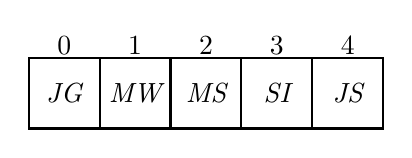
\begin{tikzpicture}[
    list/.style={
        % The shape:
        rectangle,
        % The size:
        minimum size=.9cm,
        % The border
        thick,
        draw=black,
        % The filling
        fill=white,
        % Font
        font=\itshape
    }]

    \foreach \x/\xtext/\xletters in {0/0/JG, 0.9/1/MW, 1.8/2/MS, 2.7/3/SI, 3.6/4/JS}
    {
        \node [list]  at (\x,0) {\xletters};
        \node at (\x,.6) {\xtext};
    }
\end{tikzpicture}
\end{document}
